\section{Diagramas de Estados}
\label{sec:diagramaEstados}

Es esta sección se muestran los diagramas de estados y la descripción de cada uno de ellos.

\subsection{Estados de un proyecto}

En la figura \ref{estadosProyecto} se muestran los \hypertarget{edoProy}{estados} en los que se puede encontrar un proyecto en el sistema.

\begin{figure}[H]
	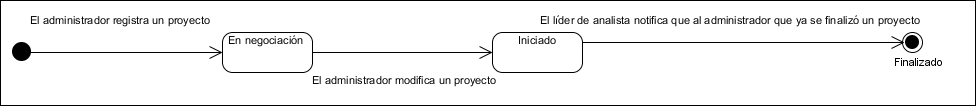
\includegraphics[scale=.50]{images/estadosProyecto}
	\caption{Estados de un proyecto}
	\label{estadosProyecto}
\end{figure}

	Cada estado se describe a continuación:

	\textbf{En negociación:} Se encuentra en este estado cuando el \hyperlink{admin}{Administrador} registra un nuevo proyecto. 
	En este estado, el el \hyperlink{admin}{Administrador} puede:
		\begin{itemize}
			\item Editar un proyecto
			\item Eliminar un proyecto
		\end{itemize}
	En este estado el {\hyperlink{jefe}{Líder de proyecto} puede:
		\begin{itemize}
			\item Gestionar los módulos de un proyecto.
			\item Gestionar las pantallas.
			\item Gestionar los términos de glosario.
			\item Gestionar las entidades.
			\item Gestionar las reglas de negocio.
			\item Gestionar los mensajes.
			\item Gestionar los actores.
			\item Gestionar los casos de uso.
		\end{itemize}
		En este estado el \hyperlink{analista}{Analista} no tiene acceso al proyecto al que esta asociado.
		Este estado es el inicio de la transición hacia el estado:
		\begin{itemize}
			\item \textbf{Iniciado:} Pasa a este estado una vez que el \hyperlink{admin}{Administrador} modifique el proyecto debido a que se aprobó el inicio del mismo.
		\end{itemize}
	
	\textbf{Iniciado:} El proyecto pasa a este estado cuando el \hyperlink{admin}{Administrador} tiene la indicación de iniciar la producción del mismo.
	En este estado el \hyperlink{admin}{Administrador} puede:
		\begin{itemize}
			\item Editar un proyecto
		\end{itemize}
	En este estado el {\hyperlink{jefe}{Líder de proyecto} puede:
		\begin{itemize}
			\item Asociar analistas a un proyecto.
			\item Gestionar los módulos de un proyecto.
			\item Asociar analistas a los módulos de un proyecto.
			\item Gestionar las pantallas.
			\item Gestionar los términos de glosario.
			\item Gestionar las entidades.
			\item Gestionar las reglas de negocio.
			\item Gestionar los mensajes.
			\item Gestionar los actores.
			\item Gestionar los casos de uso.
			\item Revisar Casos de uso.
			\item Terminar Casos de uso.
			\item Liberar Casos de uso
			\item Generar documento de análisis.
		\end{itemize}
	En este estado el \hyperlink{analista}{Analista} puede:
	\begin{itemize}
		\item Gestionar los módulos de un proyecto.
		\item Gestionar las pantallas.
		\item Gestionar los términos de glosario.
		\item Gestionar las entidades.
		\item Gestionar las reglas de negocio.
		\item Gestionar los mensajes.
		\item Gestionar los actores.
		\item Gestionar los casos de uso.
		\item Generar documento de análisis.
	\end{itemize}
	Este estado es el inicio de la transición hacia el estado:
	\begin{itemize}
		\item \textbf{Finalizado:} Pasa a este estado una vez que el \hyperlink{admin}{Administrador} sea notificado por un líder que un proyecto ha terminado.
	\end{itemize}	 
	\textbf{Finalizado:} El proyecto pasa a este estado cuando un {\hyperlink{jefe}{Líder de proyecto} notifica que un proyecto ha sido concluido, indicando que ya no se trabajará más sobre el mismo. Este estado no genera transiciones a ningún estado. 
		En este estado el \hyperlink{admin}{Administrador} puede:
		\begin{itemize}
			\item Consultar el proyecto
		\end{itemize}
		En este estado el {\hyperlink{jefe}{Líder de proyecto} puede:
			\begin{itemize}
				\item Consultar los módulos de un proyecto.
				\item Consultar las pantallas.
				\item Consultar los términos de glosario.
				\item Consultar las entidades.
				\item Consultar las reglas de negocio.
				\item Consultar los mensajes.
				\item Consultar los actores.
				\item Consultar los casos de uso.
				\item Generar documento de análisis.
			\end{itemize}
			En este estado el \hyperlink{analista}{Analista} puede:
			\begin{itemize}
				\item Consultar los módulos de un proyecto.
				\item Consultar las pantallas.
				\item Consultar los términos de glosario.
				\item Consultar las entidades.
				\item Consultar las reglas de negocio.
				\item Consultar los mensajes.
				\item Consultar los actores.
				\item Consultar los casos de uso.
				\item Consultar documento de análisis.
			\end{itemize}




\subsection{Estados de un caso de uso}

En la figura \ref{estadosCU} se muestran los \hypertarget{edoCU}{estados} en los que se puede encontrar un caso de uso en el sistema.

	\begin{figure}[H]
		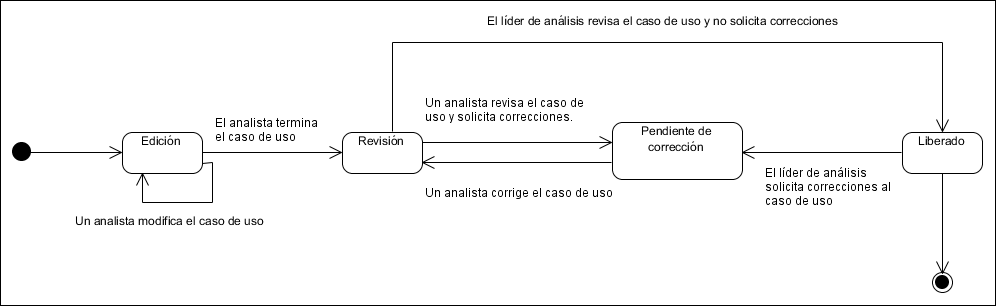
\includegraphics[scale=0.7]{images/estadosCU}
		\caption{Estados de un caso de uso}
		\label{estadosCU}
	\end{figure}

	Cada estado se describe a continuación:
	\begin{itemize}
		\item \textbf{Edición}. Un caso de uso se encuentra en este estado si:
			\begin{itemize}
				\item Un analista registra el caso de uso.
				\item Un analista modifica el caso de uso.
			\end{itemize}
	\end{itemize}
	Cuando un caso de uso se encuentra en estado \textbf{Edición}, puede ser terminado o modificado.
	
	\begin{itemize}
		\item \textbf{Revisión}. Un caso de uso se encuentra en este estado si:
		\begin{itemize}
			\item Un analista termina el caso de uso.
			\item Un analista corrige el caso de uso.
		\end{itemize}
	\end{itemize}
	Cuando un caso de uso se encuentra en estado \textbf{Revisión}, puede ser revisado por algún analista e indicar si es correcto o no.
	
	\begin{itemize}
		\item \textbf{Pendiente de corrección}. Un caso de uso se encuentra en este estado si:
		\begin{itemize}
			\item Un analista revisa el caso de uso e indica que es incorrecto.
			\item El líder de análisis decide no liberar el caso de uso.
			\item El líder de análisis solicita correcciones al caso de uso.
		\end{itemize}
	\end{itemize}
	Cuando un caso de uso se encuentra en estado \textbf{Pendiente de corrección}, puede ser corregido.
	
	\begin{itemize}
		\item \textbf{Liberado}. Un caso de uso se encuentra en este estado si:
		\begin{itemize}
			\item El líder de análisis revisa el caso de uso e indica que es correcto.
			\item El líder de análisis decide liberar el caso de uso.
		\end{itemize}
	\end{itemize}
	Cuando un caso de uso se encuentra en estado \textbf{Liberado}, el líder de análisis puede solicitar correcciones al caso de uso.